\themaN
\graphicspath{{../Ch20_La_division/Images/}}

\chapter{Les divisions}
\label{C23}


%%%%%%%%%%%%%%%%%%%%%%%%%%%%%%%%%%%%%%%%%%
\begin{prerequis}[Connaissances et compétences abordées]
   \begin{itemize}
      \item Connaître et mettre en œuvre un algorithme de calcul posé pour effectuer la division euclidienne d’un entier par un entier ; la division d’un nombre décimal (entier ou non) par un nombre entier.
      \item Connaître les critères de divisibilité par 2, 3, 5, 9 et 10.
   \end{itemize}
\end{prerequis}

\vfill

\begin{debat}[Débat : la division euclidienne] 
   Le nom de {\bf division euclidienne} est un hommage rendu à {\it Euclide} (300 av. J.-C.), mathématicien grec qui en explique le principe par soustractions successives dans son \oe uvre {\it Les éléments}. Mais elle apparait très tôt dans l'histoire des mathématiques, par exemple dans les mathématiques égyptiennes, babyloniennes et chinoises.
   \begin{center}
      \begin{pspicture}(0,1)(4,4.5)
         \psline[linewidth=1mm](2,1)(2,4)
         \psline[linewidth=1mm](2,3)(4,3)
         \textcolor{B1}{\it\large
         \rput(0.8,3.5){dividende}
         \rput(3,3.5){diviseur}
         \rput(3,2.5){quotient}
         \rput(1,1.5){reste}}
      \end{pspicture}
   \end{center}
   \bigskip
   \begin{cadre}[B2][F4]
      \begin{center}
         Vidéo : \href{https://www.youtube.com/watch?v=VWS9NyXbEyY&t=18s}{\bf Division euclidienne avec matériel multibase}, chaîne YouTube {\it Méthode Heuristique}.
      \end{center}
   \end{cadre}
\end{debat}

\vfill

\textcolor{PartieGeometrie}{\sffamily\bfseries Cahier de compétences} : chapitre 3, exercices 1 à 33.


%%%%%%%%%%%%%%%%%%%%%%%%%%%%%%%%%%%%
%%%%%%%%%%%%%%%%%%%%%%%%%%%%%%%%%%%%
\activites

\begin{activite}[Quelle opération ?]
   {\bf Objectifs :} poser une addition, une soustraction, une multiplication, une division euclidienne et une division décimale ; résoudre un problème en choisissant la bonne opération. 
   \begin{QCM}
      Pour chacun des problèmes suivants, indiquer quelle opération est en jeu, effectuer l'opération puis conclure. \medskip
      \begin{center}
         {\small
         \begin{ltableau}{0.9\linewidth}{3}
            \hline
            Énoncé & Opération & Conclusion \\ [2mm]
            \hline
            Harry Potter a acheté 8 paquets de chocogrenouilles à 180 noises le paquet. 
            \newline Combien a-t-il payé ? & & \\ [3.2cm]
            \hline
            Severus Rogue dispose de \ul{180} de philtre de confusion.
            \newline Combien de chaudrons de \ul{8} chacun peut-il faire ? & & \\ [3.2cm]
            \hline
            Voldemore mesure \ucm{180} soit \ucm{8} de plus que Dumbledore. 
            \newline Quelle est la taille de Dumbledore ? & & \\ [3.2cm]
            \hline
            Un bâton de cerisier mesure \ucm{180}. Gilderoy Lockhart découpe 8 morceaux de ce bâton pour se faire des baguettes.
            \newline Combien mesure chaque baguette ? & & \\ [3.2cm]
            \hline
            La maison Gryffondor vient de perdre 8 points suite à une mauvaise réponse en divination et elle en a maintenant 180.
            \newline  Combien avait-elle de points avant ce cours ? & & \\ [3.2cm]
            \hline
         \end{ltableau}}
         \bigskip
      \end{center}
   \end{QCM}
\end{activite}


%%%%%%%%%%%%%%%%%%%%%%%%%%%%%%%%%%
%%%%%%%%%%%%%%%%%%%%%%%%%%%%%%%%%%
\cours 


%%%%%%%%%%%%%%%%%%%%%%%%%%
\section{La division euclidienne et la division décimale}

\begin{definition}
   Effectuer une division euclidienne d'un {\bf dividende} par un {\bf diviseur}, c'est trouver deux entiers appelés {\bf quotient} et {\bf reste} tels que : \\
   \hspace*{1cm} \og dividende $=$ (diviseur $\times$ quotient) $+$ reste \fg \qquad avec \qquad reste $<$ diviseur.
\end{definition}

\begin{exemple}
   Avec une bouteille de \ucl{150} de jus, combien peut-on remplir de verres de \ucl{8} ? \\ [5mm]
   Réponse : $150 =18\times8+6$ \\
   donc, on peut remplir 18 verres de \ucl{8}.
   \correction
      \begin{pspicture}(-2.5,-0.2)(4,2.8)
         \rput(1,1.2){$\opidiv[displayintermediary=all,voperation=top]{150}{8}$}
         \psline[linecolor=A1]{->}(0.7,2.8)(0.7,2.4)
         \rput(0.7,3){\textcolor{A1}{dividende}}
         \psline[linecolor=A1]{<-}(1.9,2.3)(2.4,2.3)
         \rput[l](2.5,2.3){\textcolor{A1}{diviseur}}
         \psline[linecolor=B1]{<-}(2.2,1.7)(2.7,1.7)
         \rput[l](2.8,1.7){\textcolor{B1}{quotient}}
         \psline[linecolor=B1]{<-}(1.4,0.2)(1.9,0.2)
         \rput[l](2,0.2){\textcolor{B1}{reste}}
      \end{pspicture}
\end{exemple}

\medskip

\begin{definition}
   Effectuer la division décimale d'un {\bf dividende} par un {\bf diviseur}, c'est calculer la valeur exacte ou une valeur approchée du quotient \og dividende $\div$ diviseur \fg.
\end{definition}

\begin{exemple}
   On achète 8 CD de même prix pour \ueuro{150}, quel est le prix d'un CD ? \\ [5mm]
   Réponse : Un CD vaut \ueuro{18,75}.
   \correction
      \begin{pspicture}(-2.5,0)(4,2)
         \rput(1,1.2){\opdiv[decimalsepsymbol={,}]{150}{8}}
      \end{pspicture}
\end{exemple}

\begin{remarques}
   lorsque l'on effectue la division d'un nombre décimal par un nombre entier, au moment où on abaisse le chiffre des dixièmes dans le dividende, on pose une virgule dans le quotient. Lorsque la division \og ne s'arrête jamais \fg{} ou que le quotient comporte un grand nombre de décimales, on donne une valeur approchée du quotient.
\end{remarques}


%%%%%%%%%%%%%%%%%%%%%%%%%%
\section{Critères de divisibilité}

\begin{propriete}
   \begin{itemize}
      \item un nombre est divisible par 2 s'il se termine par 0 ; 2 ; 4 ; 6 ou 8 ;
      \item un nombre est divisible par 3 si la somme de ses chiffres est un multiple de 3 ;
      \item un nombre est divisible par 5 s'il se termine par 0 ou 5 ;
      \item un nombre est divisible par 9 si la somme de ses chiffres est un multiple de 9 ;
      \item un nombre est divisible par 10 s'il se termine par 0.
   \end{itemize}
   \vspace*{-3mm}
\end{propriete}

\begin{exemple}
      52\,362 est-il divisible par 2 ? 3 ? 5 ? 9 ? 10 ?
   \correction
      \vspace*{-5mm}
      \begin{itemize}
      \item 52\,332 se termine par 2, donc il est divisible par 2 mais pas par 5, ni par 10.
      \item $5+2+3+3+2=15$ est multiple de 3 mais pas de 9 donc, 52\,332 est divisible par 3, mais pas par 9.
    \end{itemize}
\end{exemple}


%%%%%%%%%%%%%%%%%%%%%%%%%%%%%%%%%%%%%%%%%
\exercicesbase

\begin{colonne*exercice}

%%%%%%%%%%%%%%%
\serie{Division euclidienne}

\begin{exercice}
   Effectuer les divisions euclidiennes suivantes :
   \begin{colenumerate}{2}
      \item 154 par 2.
      \item 307 par 7.
      \item 13\,758 par 25.
      \item 1\,999 par 13.
   \end{colenumerate}
\end{exercice}

\medskip
        
\begin{exercice}
   On donne les égalités : \\
   $415 = 7\times59+2$ et $56\times57 = 3\,192$. \\
   Sans effectuer de calculs, donner le quotient et le reste des divisions euclidiennes suivantes.
   \begin{colenumerate}{2}
      \item 415 par 7
      \item 3\,192 par 56
      \item 415 par 59
      \item 3\,192 par 57
   \end{colenumerate}
\end{exercice}

\medskip

\begin{exercice}
   Compléter les colonnes sans poser les divisions.
   \begin{center}
      {\hautab{1.5}
      \begin{Ctableau}{0.95\linewidth}{5}{l}
         \hline
         Dividende & 18 & & 456 & 907 \\
         \hline
         Diviseur & 5 & 15 & 45 & \\
         \hline
         Quotient & & 30 & 10 & 10 \\
         \hline
         Reste & 3 & 7 & & 7 \\
         \hline
      \end{Ctableau}}
   \end{center}
\end{exercice}

\medskip

\begin{exercice}
   Résoudre les problèmes suivants :
   \begin{enumerate}
      \item 6\,798 supporters d'un club de rugby doivent faire un déplacement en car pour soutenir leur équipe. Chaque car dispose de 55 places. Combien de cars faut-il réserver ?
      \item Des stylos sont conditionnés par boîte de 40. Marie a 2\,647 stylos. Combien lui en manque-t-il pour avoir des boîtes entièrement remplies ?
      \item Trois amis participent à une chasse au trésor et trouvent 1\,419 pièces en chocolat. Si le partage est équitable, combien de pièces en chocolat auront-ils chacun ? Kaïs arrive et leur rappelle que c'est lui qui leur a prêté sa boussole. Il exige donc d'avoir la même part que chacun des trois autres plus les pièces restantes. Combien de pièces recevra-t-il ?
   \end{enumerate}
\end{exercice}

\medskip

%%%%%%%%%%%%%%%
\serie{Division décimale}

\begin{exercice}
   Effectuer les opérations suivantes :
   \begin{colenumerate}{2}
      \item $1\,706\div5$
      \item $690\div25$
      \item $12,6\div3$
      \item $987,72\div2$
   \end{colenumerate}
\end{exercice}

\begin{exercice}
   À l'aide de la calculatrice, effectuer les divisions suivantes en donnant le résultat de la calculatrice, puis une valeur approchée à une décimale près.
   \begin{center}
      {\hautab{1.5}
      \begin{Ltableau}{0.95\linewidth}{5}{c}
         \hline
         Calcul & Résultat & Approximation \\
         \hline
         $126\div5$ & & \\
         \hline
         $1\,234\div7$ & & \\
         \hline
         $3,67\div3$ & & \\
         \hline
         $123\,456\div9$ & & \\
         \hline
         $49\,001\div25$ & & \\
         \hline
      \end{Ltableau}}
   \end{center}
\end{exercice}

\smallskip

%%%%%%%%%%%%
\serie{Critères de divisibilité}

\begin{exercice}
   Les nombres 30 ; 27 ; 246 ; 325 ; 4\,238 et 6\,129 sont-ils divisibles par 2 ? 3 ? 5 ? 9 ? Compléter le tableau.
   \begin{center}
      {\hautab{1.5}
      \begin{Ctableau}{0.95\linewidth}{7}{l}
         \hline
         & 30 & 27 & 246 & 325 & 4\,238 & 6\,129 \\
         \hline
         2 & & & & & & \\
         \hline
         3 & & & & & & \\
         \hline
         5 & & & & & & \\
         \hline
         9 & & & & & & \\
         \hline
      \end{Ctableau}}
   \end{center}
\end{exercice}

\smallskip

\begin{exercice}
   Colorier le chemin pour aller de la case 99 à la case 108 en ne passant que par des nombres divisibles par 9, horizontalement et verticalement.
   \begin{center}
   \footnotesize
      {\hautab{1.6}
      \begin{tabular}{C{0.2}|*{8}{C{0.48}|}C{0.2}}
         \cline{1-9}
         99 & 27 & 7875 & 934 & 117 & 9999 & 63 & 8321 & 69 & \\
          \cline{1-9}
         & 980 & 1116 & 128 & 9000 & 777 & 4455 & 109 & 675 & \\
         \cline{2-9}
         & 732 & 8784 & 666 & 7866 & 304 & 963 & 124 & 946 & \\
         \cline{2-9}
         & 132 & 678 & 418 & 456 & 2044 & 7272 & 1070 & 6666 & \\
         \cline{2-9}
         & 1152 & 4200 & 82 & 1035 & 3303 & 54 & 5543 & 765 & \\
         \cline{2-9}
         & 4778 & 354 & 4779 & 234 & 9001 & 1117 & 208 & 89 & \\
         \cline{2-9}
         & 810 & 888 & 7200 & 998 & 632 & 5544 & 36 & 945 & \\
         \cline{2-10}
         & 101 & 7001 & 6669 & 8757 & 207 & 1071 & 2350 & 2358 & 108 \\
         \cline{2-10}
      \end{tabular}}
   \end{center}
\end{exercice}

\smallskip

\begin{exercice}
   Je suis un nombre impair à 2 chiffres sans 2 dans mon écriture. Je ne suis pas divisible par 5 mais je suis un multiple de 9. Qui suis-je ? 
\end{exercice}

\end{colonne*exercice}


%%%%%%%%%%%%%%%%%%%%%
%%%%%%%%%%%%%%%%%%%%%
\Recreation
  
\enigme[Calculer avec Scratch]
   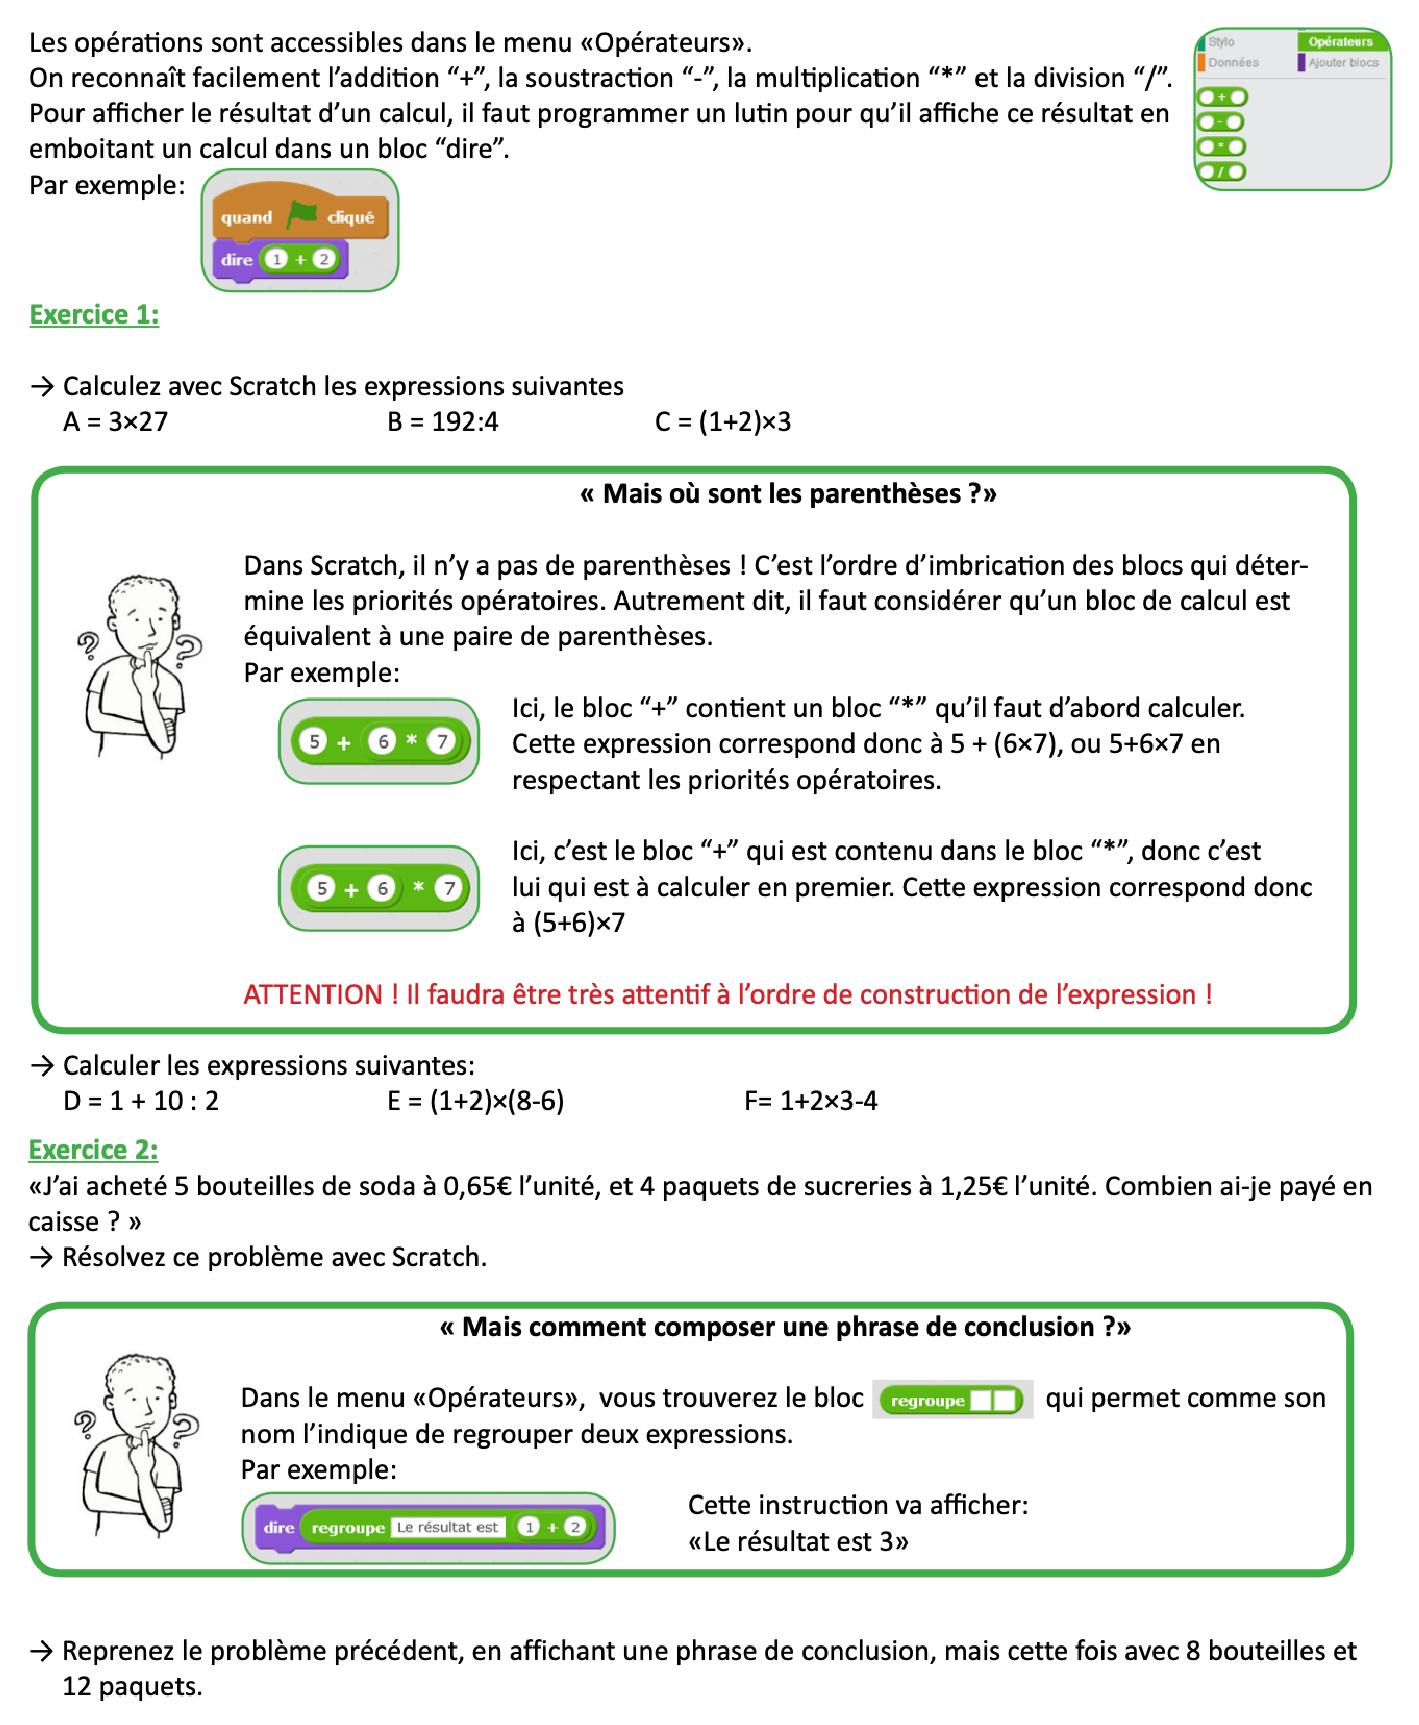
\includegraphics[width=17.5cm]{Scratch_calculer}
    \vfill\hfill {\it\footnotesize Source : \href{http://joly.vince.free.fr/Manuel_Algo/Scratch_Calculer.pdf}{Site des mathématiques de l'académie de Lille }} 
 
